%=====================================================================
%  Mityaf — Measuring Where Water Will Stand
%  Satellite-derived street-flood susceptibility for Al Madinah
%
%  Build:  latexmk -pdf mityaf.tex
%     or:  pdflatex mityaf && bibtex mityaf && pdflatex mityaf && pdflatex mityaf
%
%  To retarget a journal: replace the \documentclass line with the
%  publisher's class (e.g. elsarticle, IEEEtran, svjour3) and delete the
%  \geometry line — the body markup below is class-agnostic.
%=====================================================================
\documentclass[11pt,a4paper]{article}

\usepackage[T1]{fontenc}
\usepackage[utf8]{inputenc}
\usepackage{lmodern}
\usepackage[english]{babel}
\usepackage{geometry}
\geometry{margin=2.6cm}

\usepackage{graphicx}
\usepackage{booktabs}
\usepackage{longtable}
\usepackage{array}
\usepackage{amsmath}
\usepackage{siunitx}
\usepackage[table,dvipsnames]{xcolor}
\usepackage[most]{tcolorbox}
\usepackage{caption}
\usepackage{enumitem}
\usepackage{microtype}
\usepackage[numbers,sort&compress]{natbib}
\usepackage{setspace}
\usepackage[hidelinks,breaklinks]{hyperref}

% Manuscript spacing. Many journals require 1.5 or double spacing for the
% review copy; camera-ready is normally single. Uncomment one:
% \onehalfspacing   % ~38 pp
% \doublespacing    % ~46 pp
\singlespacing      % ~26 pp (default)

\captionsetup{font=small,labelfont=bf}
\setlist{itemsep=2pt,parsep=0pt,topsep=4pt}

%--- semantic colours -------------------------------------------------
\definecolor{accent}{HTML}{14566B}
\definecolor{warncol}{HTML}{7E5410}
\definecolor{dangercol}{HTML}{96302A}
\definecolor{okcol}{HTML}{1D5C3C}
\definecolor{rowtint}{HTML}{E9F0F4}

%--- callout environments --------------------------------------------
\newtcolorbox{keybox}[1][]{colback=okcol!6,colframe=okcol,boxrule=0pt,
  leftrule=2.5pt,arc=1pt,left=8pt,right=8pt,top=6pt,bottom=6pt,
  fonttitle=\bfseries\sffamily\small,coltitle=okcol,title={#1}}
\newtcolorbox{notebox}[1][]{colback=accent!6,colframe=accent,boxrule=0pt,
  leftrule=2.5pt,arc=1pt,left=8pt,right=8pt,top=6pt,bottom=6pt,
  fonttitle=\bfseries\sffamily\small,coltitle=accent,title={#1}}
\newtcolorbox{limitbox}[1][]{colback=warncol!7,colframe=warncol,boxrule=0pt,
  leftrule=2.5pt,arc=1pt,left=8pt,right=8pt,top=6pt,bottom=6pt,
  fonttitle=\bfseries\sffamily\small,coltitle=warncol,title={#1}}
\newtcolorbox{trapbox}[1][]{colback=dangercol!6,colframe=dangercol,boxrule=0pt,
  leftrule=2.5pt,arc=1pt,left=8pt,right=8pt,top=6pt,bottom=6pt,
  fonttitle=\bfseries\sffamily\small,coltitle=dangercol,title={#1}}

\newcommand{\Mityaf}{Mityaf}
\newcommand{\ttt}[1]{\texttt{#1}}

%=====================================================================
\title{\bfseries Measuring Where Water Will Stand\\[4pt]
  \large\normalfont\itshape Satellite-derived street-flood susceptibility
  for a city that has never recorded a flood}

\author{\Mityaf{} Project\\[2pt]
  \small Barmajan Al Munawwarah 2026}
\date{}

\begin{document}
\maketitle

\begin{abstract}
\noindent
Al Madinah receives a millimetre or more of rain on roughly \SI{2.3}{\percent} of days
--- about eight days a year --- and those eight days are what close its streets. Because rain is rare, the
city never accumulates an operational memory of where water stands, so each storm is
handled as though it were the first. Response is reactive: a street floods, somebody
reports it, a tanker arrives. A neighbourhood that does not complain never appears on
any map.

This paper describes a system that ranks all \num{30337} street segments in the city by
their susceptibility to standing water, using only a digital elevation model and an
open street map --- no ground sensors, no local flood records, and no satellite imagery
of flooding itself. The central methodological problem is that \emph{Al Madinah has no
labelled flood incidents at all}. We therefore do not train a model on Al Madinah.
Instead we ask a narrower, testable question: do the nine features computable for
Al Madinah predict street flooding in cities that \emph{do} have records? Using
\num{101756} geolocated citizen reports from New York and Chicago, under spatially
blocked cross-validation and a leave-one-city-out transfer test, the answer is yes ---
\num{1.44}$\times$ and \num{1.45}$\times$ over baseline within cities, and
\num{1.24}$\times$ and \num{1.30}$\times$ when transferred to a city the model has
never seen.

We explain, from first principles, where the elevation data comes from and how a radar
satellite measures ground height; what each of the nine features means physically; why
accuracy is the wrong metric and what PR-AUC measures instead; why the choice of
negative samples mattered more than the choice of algorithm; and what the resulting
rankings can and cannot tell a municipal engineer.

\smallskip
\noindent\textbf{Keywords:} pluvial flooding; flood susceptibility; digital elevation
model; gradient boosting; spatial cross-validation; transfer learning; Al Madinah.
\end{abstract}

\tableofcontents
\newpage

%=====================================================================
\section{Introduction}\label{sec:intro}

\subsection{The situation}
When rain falls on a city, not all of it reaches a drain. Some of it stands. And it
stands in particular places that repeat every season: a closed depression with no
outlet, a street lower than its surroundings, a point where the runoff of many streets
above converges.

In Al Madinah this happens on about eight days a year; the city lies in an arid zone
where rain of a millimetre or more --- the World Meteorological Organization's threshold
for a rain day --- falls on roughly \SI{2.3}{\percent} of days. Days heavy enough to
actually stand on a road, above \SI{5}{\milli\metre}, are fewer still: two or three a
year. That rarity is usually described as a mitigating factor. It is the opposite. Because storms are rare, the municipality
never builds an institutional memory of where water collects. There is no dataset of
past ponding locations, no accumulated map, no list. Each rain event is therefore
managed from scratch, and the knowledge of where the water went evaporates with the
water.


\begin{notebox}[How many rainy days, exactly?]
A ``rainy day'' is not a self-defining quantity --- it depends entirely on the
threshold you count at. The World Meteorological Organization counts a day as a
rain day when it receives \SI{1}{\milli\metre} or more, and that is the threshold
used throughout this paper. Because the distinction changes the headline figure by
a factor of three, we verified it against five independent sources for the city
centroid ($24.47^\circ$N, $39.61^\circ$E):

\smallskip
{\centering\footnotesize
\begin{tabular}{@{}llrrrr@{}}
\toprule
Source & Kind & $\ge$0.1 & $\ge$1 & $\ge$5 & Total \\
\midrule
Open-Meteo ERA5, 2015--2026 & Reanalysis & 21.3 & \textbf{8.2} & 2.7 & \SI{53.8}{\milli\metre} \\
Open-Meteo ERA5-seamless, 2015--2025 & Reanalysis & 24.7 & \textbf{7.9} & 1.6 & \SI{39.3}{\milli\metre} \\
NASA POWER (MERRA-2), 2015--2025 & Reanalysis & 13.5 & \textbf{6.9} & 2.5 & \SI{50.7}{\milli\metre} \\
Meteostat station OEMA & Gauge, 33\% complete & 21.9 & 12.1 & 5.1 & \SI{96.8}{\milli\metre} \\
Published climate normals & Compilation & 11.7--24.6 & --- & --- & 44--\SI{60}{\milli\metre} \\
\bottomrule
\end{tabular}
\par}

\smallskip
Days per year at the city centroid, by precipitation threshold in millimetres.
The three reanalyses agree closely at the WMO threshold --- 6.9 to 8.2 days ---
and that agreement is where ``about eight days'' comes from. The airport gauge
reports more, but only a third of its days since 2015 carry a precipitation value
at all and its annual total is roughly double that of the reanalyses, so its wet
days are almost certainly over-represented; we report it for completeness and do
not rely on it.

\smallskip
The threshold matters more than the choice of source. Counting \emph{any}
measurable trace roughly triples the count, to between thirteen and twenty-five
days --- but a few tenths of a millimetre does not stand on a street. Days above
\SI{5}{\milli\metre}, which do, number \textbf{two to three a year}. Read that way
the scarcity argument below is sharper, not softer.
\end{notebox}

What fills the vacuum is the complaint. A street floods; a resident is affected; the
resident reports it through the Balady+ platform or the 940 line; a tanker is dispatched
to pump the water away. The response is competent and it is entirely reactive. It begins
after the damage, and it acts on the subset of locations that somebody chose to report.

\begin{keybox}[The gap this paper addresses]
A municipality that owns \SI{5280}{\kilo\metre} of street network and a finite number of
crews needs to know \emph{where to look first} --- before the season, not after the
storm. That is a ranking problem, not a forecasting problem, and it is solvable with
data that is free and globally available.
\end{keybox}

\subsection{Why this is methodologically hard}
The obvious approach would be to collect Al Madinah's historical flood records and train
a model on them. This is impossible: \textbf{those records do not exist}. Nobody surveys
the city during a storm and writes down where the water stood. There is no labelled
dataset, which means there is nothing to train on and --- more importantly --- nothing
to test against.

This constraint is usually hidden. A model can always be fitted to something, and a
number can always be reported. But a model trained without labels and then declared
``accurate'' has been measured against nothing at all. Rather than conceal the problem,
we let it define the research question. Instead of asking \emph{how do we build a model
for Al Madinah?}, we asked:

\begin{notebox}
Do the features computable for Al Madinah --- from terrain and urban form alone, with no
field data whatsoever --- actually predict street flooding in cities that \emph{do} have
field data?
\end{notebox}

If the answer is no, the product is built on sand and should not be built. If the answer
is yes, then what transfers to Al Madinah is the \emph{shape} of the model --- the
feature definitions, the sampling rule, the validation protocol, the physical
relationships --- and explicitly \emph{not} the fitted weights. Sections
\ref{sec:validation}--\ref{sec:results} describe how we tested that, and what it cost.

\subsection{What is not claimed}
Precision about claims matters more here than in most domains, because the failure mode
is not an inaccurate map --- it is a municipality reallocating budget on the basis of
one. Four claims are explicitly \emph{not} made:

\begin{itemize}
  \item \textbf{Not a forecast.} The model does not say a street will flood on a given
        date. It ranks susceptibility, a property of place, not of weather.
  \item \textbf{Not a depth estimate.} Nothing distinguishes \SI{5}{\centi\metre} of
        water from half a metre.
  \item \textbf{Not a flash-flood or wadi model.} Section \ref{sec:types} draws this
        boundary carefully, because the most publicised Saudi flood events are of exactly
        the kind this system does \emph{not} address.
  \item \textbf{Not superior to published work.} Section \ref{sec:compare} explains why
        no such comparison is meaningful given the state of the literature.
\end{itemize}

%=====================================================================
\section{Background: Urban Pluvial Flooding}\label{sec:background}

\subsection{Pluvial, fluvial, and flash flooding}\label{sec:types}
\textbf{Fluvial flooding} occurs when a river or channel exceeds its banks, driven by
the water balance of an entire upstream catchment. \textbf{Flash flooding} is a rapid,
high-energy wave travelling down a normally dry channel --- in Arabia, a \emph{wadi}. It
carries debris, moves vehicles, and destroys infrastructure; it is the phenomenon behind
almost every fatal Saudi flood event in the public record. \textbf{Pluvial flooding} ---
also called surface-water or nuisance flooding --- is rain that falls on a surface and
cannot drain away from where it lands. No river is involved; the water is local, usually
shallow, and its location is governed by very local topography and by how much of the
surface is impervious. This third phenomenon is the subject of this paper.

\begin{figure}[htbp]\centering
  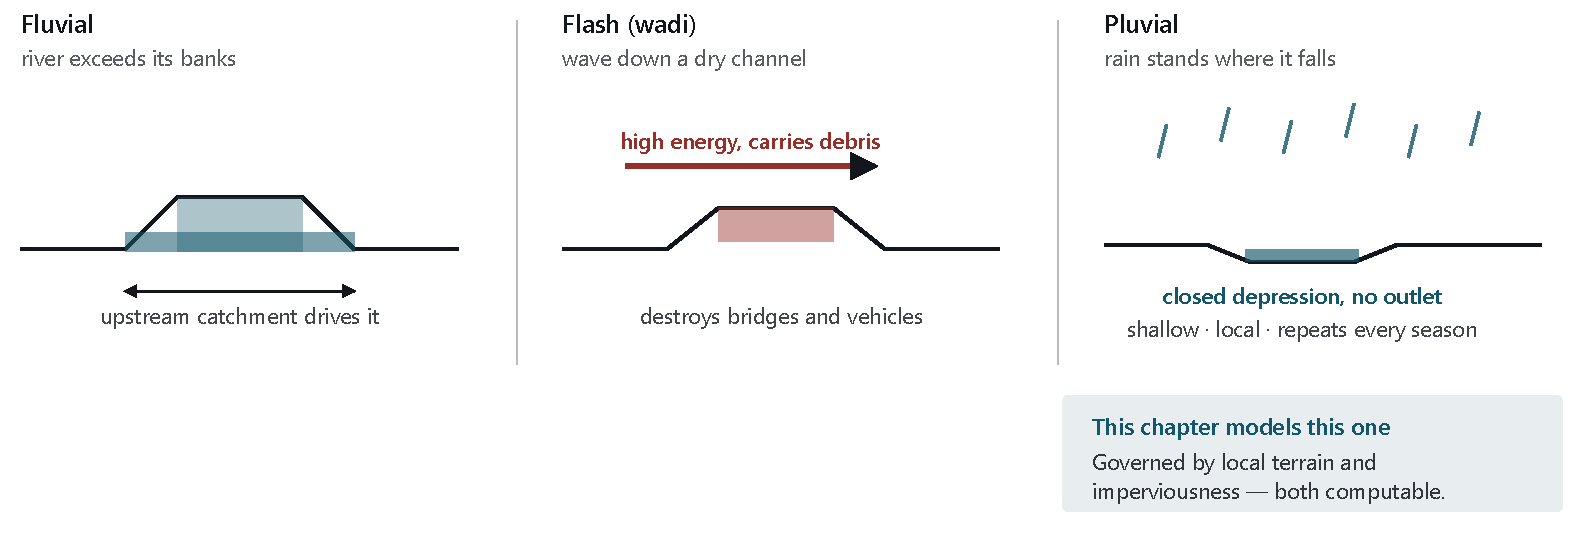
\includegraphics[width=\linewidth]{figures/fig01-flood-types.pdf}
  \caption{Three phenomena, one word. Fluvial and flash flooding are driven by upstream
  catchment hydraulics and channel dynamics. Pluvial flooding is governed by whether the
  water that lands on a spot can leave it --- a function of local depression depth and
  surface imperviousness. Only the third is predictable from a static elevation model and
  a street map.}
  \label{fig:types}
\end{figure}

\subsection{The Saudi record}
Saudi Arabia's documented flood disasters are overwhelmingly of the second kind
(Table~\ref{tab:events}). They explain why flood risk is a national priority, and they
mark the boundary of what this work addresses.

\begin{table}[htbp]\centering\small
\caption{Documented Saudi flood events.}\label{tab:events}
\begin{tabular}{@{}p{2.6cm}p{8.2cm}p{2.2cm}@{}}
\toprule
\textbf{Event} & \textbf{Documented outcome} & \textbf{Type}\\
\midrule
Jeddah, Nov 2009 & 122 killed, 350+ missing; \SI{>70}{\milli\metre} in four hours;
  3{,}000+ vehicles swept away or damaged; described by civil defence as the worst in
  27 years & Flash / urban\\
Jeddah, Jan 2011 & \SI{111}{\milli\metre} in three hours; $\sim$10 killed; 1{,}451
  rescued by ground teams and 498 by helicopter. Combined 2009+2011 damages
  $\approx$ US\$3\,bn & Flash / urban\\
\rowcolor{rowtint}
Jazan, 4 Aug 2024 & Heaviest rain in five years. A section of the bridge linking Sabya
  and Abu Arish over Wadi Jazan collapsed; two vehicles fell --- one death, five
  injuries. Wadi Al-Khams swept away a man and his wife; she died, he died two days
  later in intensive care. \textbf{Three deaths total.} Water entered the ground floors
  of King Fahd Central Hospital; the National Transport Safety Center opened an
  investigation & Flash (wadi)\\
Al Madinah, Aug 2024 & Floods described as unprecedented inundated streets and
  neighbourhoods; a child was rescued from a torrent; civil defence responded to a
  vehicle swept away in Wadi Al-Uwaynah --- one rescued, one recovered deceased
  & Flash + pluvial\\
\bottomrule
\end{tabular}
\end{table}

\begin{trapbox}[Boundary statement]
The Jazan bridge collapse and the Jeddah disasters are \textbf{wadi flash floods}. This
system would not have predicted or prevented any of them. It does not model channel
hydraulics, wave propagation, bridge scour, or structural safety. Citing these events as
motivation while implying the model addresses them would be a misrepresentation.

The connection that \emph{is} real: the same terrain descriptors used here --- height
above nearest drainage, closed-depression depth, flow accumulation --- also determine
which streets lie in the path of, or in depressions fed by, wadi overflow. The tool is
relevant to the same hazard family at a different scale, with a narrower claim.
\end{trapbox}

\subsection{Al Madinah's hydrology}
Seven wadis cross Al Madinah. Wadi Al-Aqiq is the most storied. Wadi Bathan runs through
the centre toward the north-west and is formed from four smaller valleys. Wadi Mudhainib
is a branch of Bathan, sharing its source at Dhu al-Jadr. Wadi Qanat is the largest,
originating from Wadi Waj near Taif. Al-Aqiq, Qanat and Bathan converge at Al-Zaghabah
north-west of the city to form Wadi Al-Hamd.

A city built across seven drainage lines has a terrain surface whose natural flow paths
run through, not around, the urban fabric. Notably, \emph{Wadi Mudhainib is also the name
of a residential district}, and it appears in this system's output among the ten most
exposed districts, with 128 segments in the high or critical bands --- a neighbourhood
named after a valley, surfacing in a risk ranking computed from terrain alone.

\subsection{Why rarity makes the problem worse}
Intuitively, a city that rarely floods has a smaller problem. Operationally the reverse
holds:

\begin{enumerate}
  \item \textbf{No institutional memory forms.} Learning requires repetition close enough
        in time to connect cause and effect. Eight events a year across a
        \SI{545}{\kilo\metre\squared} city means a given street segment may flood once in
        several years --- too sparse for a reliable mental map.
  \item \textbf{No dataset accumulates.} Rare events produce few records, and few records
        mean no basis for statistical learning. This is precisely the constraint that
        shaped this study.
  \item \textbf{Infrastructure is sized for the average, tested by the maximum.} The
        heaviest day in Al Madinah's rainfall archive is \SI{65.6}{\milli\metre}.
\end{enumerate}

Climate projections sharpen this. Studies of Saudi rainfall report intensifying extremes
alongside declining annual totals \citep{almazroui2020,escwa2017} --- fewer rain days,
heavier peaks. Meanwhile the Ministry of Municipalities and Housing laid more than
\num{454000} linear metres of stormwater drainage in 2024 alone, against \num{291000} in
2023, for a programme total exceeding eight million linear metres \citep{momah2025}. Yet
no independent instrument measures whether any given scheme worked after commissioning;
success is assessed from the contractor's own report.

%=====================================================================
\section{Related Work}\label{sec:related}

\subsection{Terrain indices: the TOPMODEL lineage}
The idea that the shape of the land predicts where water accumulates is not new.
TOPMODEL \citep{beven1979} introduced the \textbf{Topographic Wetness Index} (TWI),
combining upslope contributing area with local slope:

\begin{equation}
\mathrm{TWI} = \ln\!\left(\frac{a}{\tan\beta}\right)
\label{eq:twi}
\end{equation}

\noindent where $a$ is upslope contributing area per unit contour width and $\beta$ is
local slope. A large upslope area delivers much water; a shallow slope removes it slowly.

Computing $a$ requires flow directions. The standard method is the \textbf{D8} algorithm
\citep{ocallaghan1984}: each cell drains to whichever of its eight neighbours lies
steepest downhill. D8 fails at \emph{pits} --- cells lower than all neighbours --- where
routing terminates. The efficient remedy is \textbf{priority-flood}
\citep{barnes2014}, which floods the surface inward from the boundary using a priority
queue. Crucially, the amount by which each cell is raised is itself meaningful: it is the
depth of the closed depression at that point.

A second descriptor, \textbf{HAND} (Height Above Nearest Drainage), was introduced by
\citet{renno2008} and developed by \citet{nobre2011}. Rather than absolute elevation, it
measures how high a point sits above the nearest channel draining it, normalising terrain
to the local water level.

\subsection{Terrain indices in urban settings}
Transferring these indices from catchments to cities is not automatic. Urban surfaces are
engineered: the flow path a DEM implies may be interrupted by a kerb, a culvert, or a
storm drain the elevation model cannot see. \citet{kelleher2020} examined precisely
whether topographic indices identify pluvial flooding locations in urban landscapes and
found the relationship real but weaker and noisier than in natural catchments, because
subsurface drainage is invisible to terrain analysis. This finding sets a ceiling on
achievable performance and explains why our results are modest multiples of baseline
rather than the near-perfect scores appearing in some susceptibility studies.

\subsection{Machine learning for flood susceptibility}
A large literature applies statistical and machine-learning classifiers to flood
susceptibility mapping over stacks of terrain and land-cover rasters
\citep{tehrany2014,dano2019}. Tree ensembles dominate recent work because the
relationships are strongly non-linear and interacting. \textbf{Gradient boosting} as
implemented in XGBoost \citep{chen2016xgboost} is the method used here; its practical
advantages are that it handles heterogeneous numeric features without scaling, tolerates
class imbalance through instance weighting, and exposes a per-feature \ttt{gain}
attribution that can be shown to an engineer as a reason.

\subsection{Citizen reports as ground truth}
The absence of authoritative flood inventories has pushed researchers toward
crowd-sourced and administrative complaint data. New York City's 311 archive has become
a reference dataset; several studies use its street-flooding descriptor to study spatial
patterns of urban pluvial flooding \citep{agonafir2022understanding,agonafir2022ml}.
These datasets have a well-understood weakness, returned to in Section \ref{sec:limits}:
a complaint records where somebody \emph{reported} water, which is not the same as where
water \emph{was}.

\subsection{Trap one: spatial autocorrelation}
Terrain variables are strongly spatially autocorrelated --- adjacent cells share slope,
catchment, and imperviousness almost by definition. If training and test sets are formed
by random splitting, neighbouring and nearly identical cells land on both sides, and the
reported metric measures interpolation rather than prediction. \citet{roberts2017} set
out blocking strategies for this situation, and \citet{ploton2020} demonstrated that
spatially naive validation can make ecological models appear excellent while their true
out-of-sample power is close to nil.

\begin{trapbox}[Why this matters when reading any susceptibility paper]
A published ROC-AUC of \num{0.95} under random $k$-fold and a PR-AUC of \num{0.40} under
spatial blocking can describe the \emph{same model on the same data}. When comparing
across studies, the validation protocol matters more than the headline number.
\end{trapbox}

\subsection{Trap two: presence-only data}
Complaint archives are \textbf{presence-only}: they record where flooding was reported
and say nothing about where it was absent. Negatives must therefore be constructed, and
how they are constructed determines what question the model answers. This problem is best
developed in species distribution modelling. \citet{phillips2009} showed that sample
selection bias in presence-only data systematically distorts fitted models, and
\citet{barbetmassin2012} gave practical guidance on choosing pseudo-absences: draw them
from the same environmental domain in which presences could have been observed, or the
classifier learns the sampling process instead of the phenomenon. Section
\ref{sec:negatives} shows what this meant concretely --- and it mattered more than the
choice of algorithm.

\subsection{Evaluation under class imbalance}
When positives are a minority, accuracy becomes meaningless and ROC-AUC misleadingly
flattering, because the large number of true negatives dominates the false positive rate.
\citet{davis2006} established the formal relationship between ROC and precision--recall
space, and \citet{saito2015} demonstrated that the precision--recall plot is the more
informative of the two on imbalanced data. Section \ref{sec:metrics} develops this from
first principles.

\subsection{Where this work sits}
The contribution is not a new algorithm or terrain index. It is a \emph{transfer} result
under a deliberately harsh protocol, addressing a situation the literature rarely
confronts: a target city with \textbf{zero labels}. The question --- can a feature set
computable for an unlabelled city be validated on labelled cities, and how much
predictive power survives the move --- is, as far as we can determine, not answered
elsewhere for urban pluvial flooding.

%=====================================================================
\section{Data}\label{sec:data}

Every input is free, open, and globally available. This is a design constraint, not a
convenience: a feature that cannot be reproduced for Al Madinah is useless no matter how
well it performs in New York.

\subsection{Elevation: from radar to raster}\label{sec:dem}
Six of the nine features derive from a \emph{single file}.

\begin{table}[htbp]\centering\small
\caption{Provenance of the elevation data.}\label{tab:dem-prov}
\begin{tabular}{@{}p{3.6cm}p{9.4cm}@{}}
\toprule
Mission & \textbf{TanDEM-X} --- two German radar satellites in close formation
  \citep{krieger2007tandemx}\\
Operators & German Aerospace Center (DLR) with Airbus Defence and Space\\
Technique & Bistatic interferometric SAR (InSAR) in the X band\\
Acquisition & 2011--2015\\
Processing & Edited into WorldDEM: water flattened, river courses made consistent,
  coastlines edited, implausible terrain removed\\
\rowcolor{rowtint}
Free derivative used & \textbf{Copernicus DEM GLO-30}, the \SI{30}{\metre} public
  release \citep{esa2022copdem}\\
\bottomrule
\end{tabular}
\end{table}

\paragraph{How a radar satellite measures ground height.}
This is \textbf{not a photograph}. No camera is involved and the measurement does not
depend on sunlight. Two spacecraft fly a few hundred metres apart. One transmits a
microwave pulse toward the ground; both receive the echo. Because the receivers sit at
slightly different positions, the returning wave arrives at each with a slightly
different \emph{phase}. That phase difference is a function of path-length difference,
and path length depends on how far away the ground is. Measured across a scene, it
resolves to the height of every point on the surface. Microwaves pass through cloud and
need no illumination, which is why global coverage was achievable at all.

\begin{figure}[htbp]\centering
  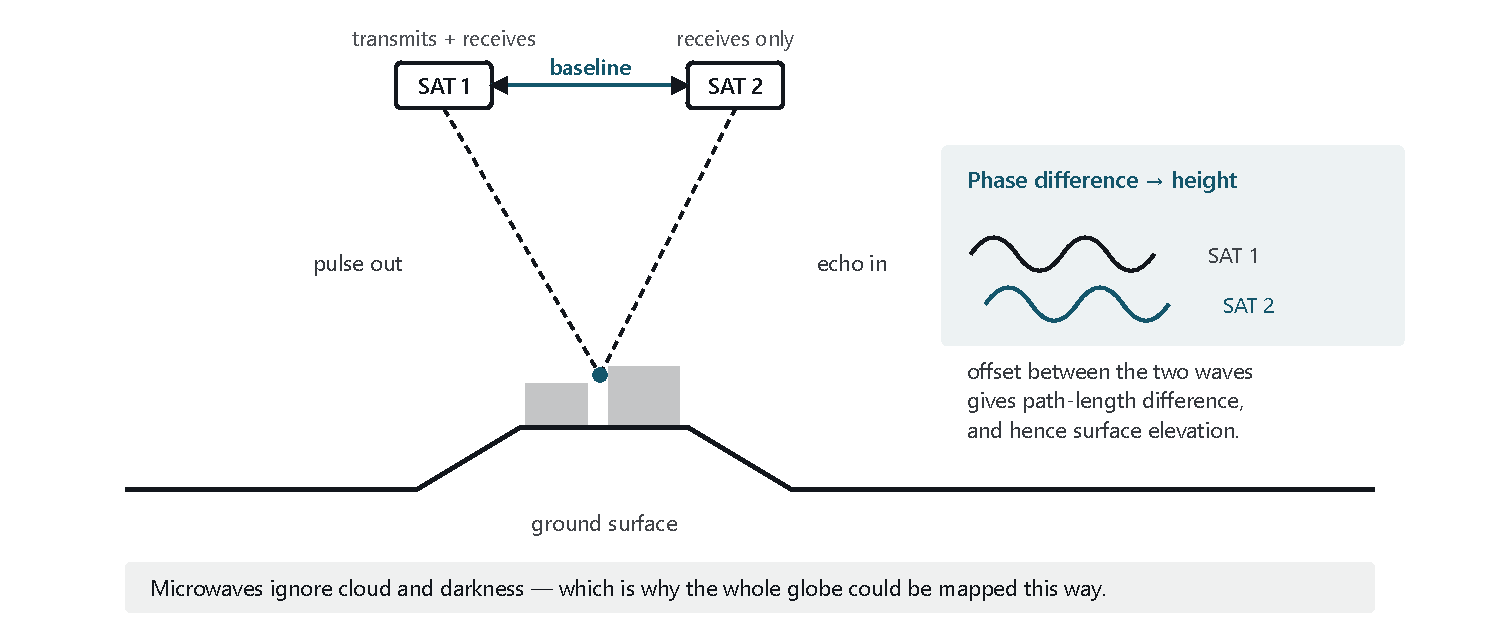
\includegraphics[width=\linewidth]{figures/fig02-insar.pdf}
  \caption{Bistatic InSAR, the measurement behind every terrain feature in this model.
  One pulse, two receivers a known distance apart. The phase offset between the returns
  encodes the difference in path length, which resolves to surface height. The output is
  not an image of the ground but a grid of elevation numbers.}
  \label{fig:insar}
\end{figure}

\begin{table}[htbp]\centering\small
\caption{Physical characteristics of the Copernicus DEM GLO-30 product.}\label{tab:dem-file}
\begin{tabular}{@{}p{4.4cm}p{8.6cm}@{}}
\toprule
Format & Cloud-Optimized GeoTIFF (COG), 32-bit floating point\\
Tiling & $1^{\circ}\times1^{\circ}$ tiles\\
Coordinate system & WGS84-G1150, \ttt{EPSG:4326}\\
Vertical datum & EGM2008 geoid, \ttt{EPSG:3855} (not the ellipsoid)\\
Absolute vertical accuracy & better than \SI{4}{\metre} at \SI{90}{\percent} linear error\\
Al Madinah tile size & \SI{41.9}{\mega\byte}\\
\rowcolor{rowtint}
Access & Public AWS bucket --- no key, no account, no cost\\
\bottomrule
\end{tabular}
\end{table}

\begin{quote}\ttfamily\footnotesize
https://copernicus-dem-30m.s3.amazonaws.com/\\
\hspace*{1em}Copernicus\_DSM\_COG\_10\_N24\_00\_E039\_00\_DEM/\\
\hspace*{1em}Copernicus\_DSM\_COG\_10\_N24\_00\_E039\_00\_DEM.tif
\end{quote}

Tile names derive from the south-west corner, so Al Madinah --- spanning
$24.36^{\circ}$--$24.58^{\circ}$\,N and $39.50^{\circ}$--$39.72^{\circ}$\,E --- falls
entirely inside \ttt{N24\_00\_E039\_00}. One HTTP request retrieves the terrain basis for
the entire study.

\paragraph{Is it updated? No.}
The data is a snapshot, not a stream. Acquisition ended in 2015. Nine releases issued
between 2019 and 2024 are corrective and refinement maintenance of the same measurements,
not new capture. Valleys, depressions and slopes do not change measurably in a decade,
but \textbf{construction after 2015 is absent from the model} --- a genuine limitation in
a rapidly expanding city.

\subsection{The most important limitation: surface, not ground}\label{sec:dsm}
Copernicus DEM is a \textbf{DSM} --- a Digital \emph{Surface} Model. It records the top
of whatever the radar hit, \emph{including buildings and vegetation}. It is not a DTM of
the bare earth. Water does not flow across rooftops, so computing flow accumulation over
a DSM in a dense neighbourhood routes some water over buildings rather than along the
streets between them. This is the largest source of physical error in the feature set.

Rather than note the concern and move on, we measured it against FABDEM
\citep{hawker2022fabdem}, a bare-earth correction of the same product
(Table~\ref{tab:dsm-dtm}).

\begin{table}[htbp]\centering\small
\caption{Measured DSM--DTM discrepancy over Al Madinah, computed via Google Earth Engine.}
\label{tab:dsm-dtm}
\begin{tabular}{@{}lrp{7.4cm}@{}}
\toprule
Percentile & Surface $-$ bare earth & Interpretation\\
\midrule
Median & \SI{0.18}{\metre} & Half the city is open desert --- essentially no difference\\
\rowcolor{rowtint}
90th & \SI{2.44}{\metre} & The built decile: surface sits $\sim$\SI{2.4}{\metre} above ground\\
\rowcolor{rowtint}
99th & \SI{5.44}{\metre} & Densest \SI{1}{\percent} --- precisely where street flooding occurs\\
\bottomrule
\end{tabular}
\end{table}

\begin{figure}[htbp]\centering
  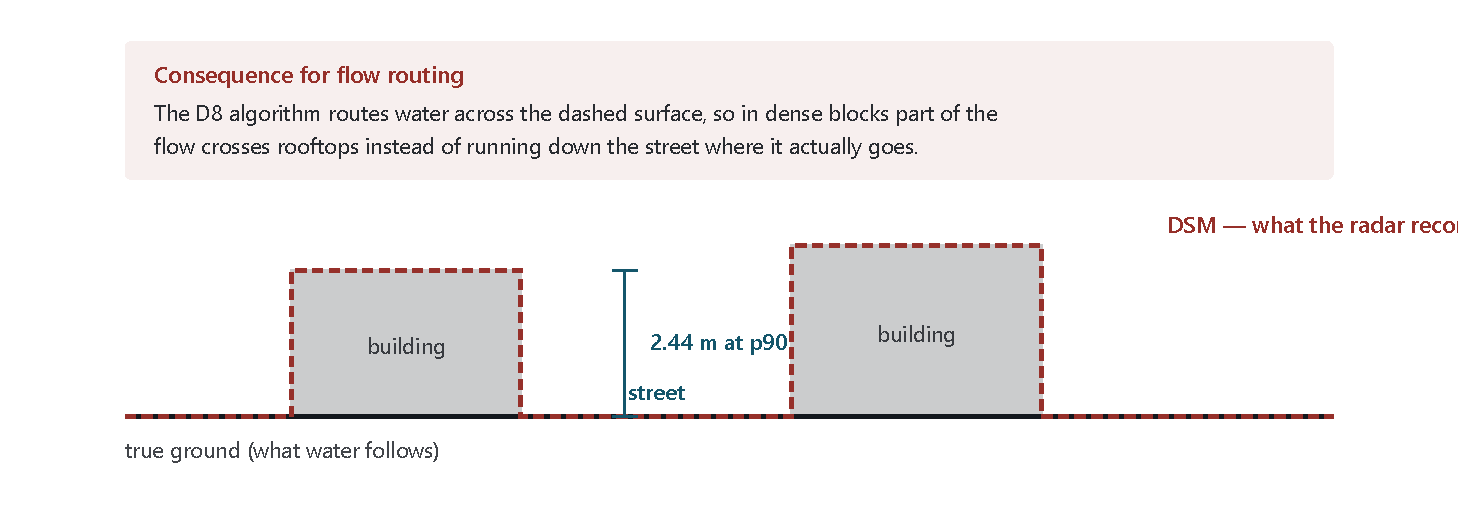
\includegraphics[width=\linewidth]{figures/fig03-dsm-dtm.pdf}
  \caption{Why a surface model misroutes urban water. The radar recorded the tops of
  buildings, so the elevation grid bridges over city blocks. Flow accumulation computed on
  it partly ignores the street canyons that actually carry runoff. The measured gap is
  negligible across open desert but reaches \SI{2.44}{\metre} in the built decile.}
  \label{fig:dsmdtm}
\end{figure}

FABDEM removes buildings and trees using machine learning, reducing mean absolute
vertical error in built-up areas from \SI{1.61}{\metre} to \SI{1.12}{\metre}. It is free
under CC BY-NC-SA 4.0 --- \emph{non-commercial} --- so a paid municipal deployment would
require a licence. Higher-resolution commercial options exist: Airbus WorldDEM at
\SI{12}{\metre} and WorldDEM Neo at \SI{5}{\metre}.

\subsection{Vector data: OpenStreetMap}
Three features and the entire spatial unit definition come from OpenStreetMap
\citep{osm}, queried through the Overpass API: road centrelines with their \ttt{highway}
classification, street names, and administrative district boundaries. OSM is the only
globally consistent, freely licensed street network whose classification scheme means the
same thing in New York, Chicago and Al Madinah --- and that consistency is what makes
cross-city transfer testable at all.

\subsection{Labels: 311 complaint archives}
Al Madinah has no labels, so they come from two American cities whose complaint systems
use a descriptor meaning, literally, \emph{standing water on a street surface}
(Table~\ref{tab:labels}).

\begin{table}[htbp]\centering\small
\caption{Ground-truth labels. Both archives are open, keyless, ongoing, and served
through the same Socrata API.}\label{tab:labels}
\begin{tabular}{@{}lllr@{}}
\toprule
City & Source & Descriptor & Reports\\
\midrule
New York & \ttt{data.cityofnewyork.us} & \ttt{Street Flooding (SJ)} & \num{21287}\\
Chicago & \ttt{data.cityofchicago.org} & \ttt{Water On Street Complaint} & \num{80469}\\
\midrule
\rowcolor{rowtint}
\textbf{Total} & & & \textbf{\num{101756}}\\
\bottomrule
\end{tabular}
\end{table}

The descriptor match matters: these are not river floods, not basement flooding, not
building inundation --- they are reports of water standing on a road, the same phenomenon
the model is asked to rank in Al Madinah.

\paragraph{Why two cities and not one.}
Spatial splitting within a single city answers \emph{does the model generalise across
neighbourhoods?} It cannot answer \emph{does it generalise across cities?}, because
within one city drainage design, climate and reporting culture are held constant --- and
those are precisely what differ in Al Madinah. Two further cities were examined and
rejected, recorded so the check is not repeated: San Francisco has no street-flooding
category, only a building-level descriptor; Baltimore's Socrata resource did not respond.

\subsection{What the model actually sees}

\begin{notebox}[There are no images in this model]
No satellite photograph, no aerial image, no picture of a flood. The model sees a
\textbf{table}: one row per \SI{200}{\metre} cell, nine numeric columns, and a 0/1 label.
The rasters are inputs to feature computation, not inputs to the classifier.
\end{notebox}

\begin{table}[htbp]\centering\small
\caption{Training matrix schema --- nine continuous predictors and one binary target.
All values are numeric; there are no categorical, text, or image inputs.}\label{tab:schema}
\begin{tabular}{@{}llll@{}}
\toprule
Column & Type & Units & Derived from\\
\midrule
\ttt{slope} & float32 & degrees & DEM gradient\\
\ttt{sink} & float32 & metres & DEM, priority-flood\\
\ttt{logacc} & float32 & log(cell count) & DEM, D8 accumulation\\
\ttt{twi} & float32 & dimensionless & DEM, Eq.~\eqref{eq:twi}\\
\ttt{hand} & float32 & metres & DEM + derived drainage network\\
\ttt{relelev} & float32 & metres & DEM $-$ $17\times17$ moving mean\\
\ttt{road\_density} & float32 & km/km\textsuperscript{2} & OSM road geometry\\
\ttt{major\_frac} & float32 & ratio 0--1 & OSM highway class\\
\ttt{load\_per\_road} & float32 & log ratio & DEM accumulation $\div$ OSM road length\\
\midrule
\rowcolor{rowtint}
\ttt{label} & int 0/1 & --- & 311 complaint present in cell\\
\bottomrule
\end{tabular}
\end{table}

%=====================================================================
\section{Exploratory Data Analysis}\label{sec:eda}

\subsection{Label geography --- and a result hiding in it}
New York's \num{21287} complaints distribute very unevenly across the five boroughs
(Table~\ref{tab:boroughs}).

\begin{table}[htbp]\centering\small
\caption{Complaint distribution by New York borough.}\label{tab:boroughs}
\begin{tabular}{@{}lrl@{}}
\toprule
Borough & Complaints & Character\\
\midrule
Queens & \num{8169} & Large, mixed density\\
Brooklyn & \num{6744} & Dense, largely low-rise\\
Staten Island & \num{3117} & Suburban, hilly\\
Bronx & \num{1757} & Dense, hilly\\
\rowcolor{rowtint}
\textbf{Manhattan} & \textbf{\num{1465}} & Densest and flattest --- \textbf{fewest complaints}\\
\bottomrule
\end{tabular}
\end{table}

Manhattan is the densest and flattest borough and produces the \emph{fewest}
street-flooding complaints. On a purely topographic account this should not happen. The
literature attributes it to sewer design: Manhattan runs a \textbf{combined sewer} system
of substantial capacity, whereas the outer boroughs largely use separate storm sewers.

\begin{keybox}[The methodological lesson, extracted early]
Drainage \emph{design} --- invisible to any elevation model --- governs outcomes as
strongly as terrain does. This single observation is why transfer performance is reported
separately, and why the fitted \textbf{weights} are declared non-transferable while the
feature \textbf{definitions} are.
\end{keybox}

\begin{figure}[htbp]\centering
  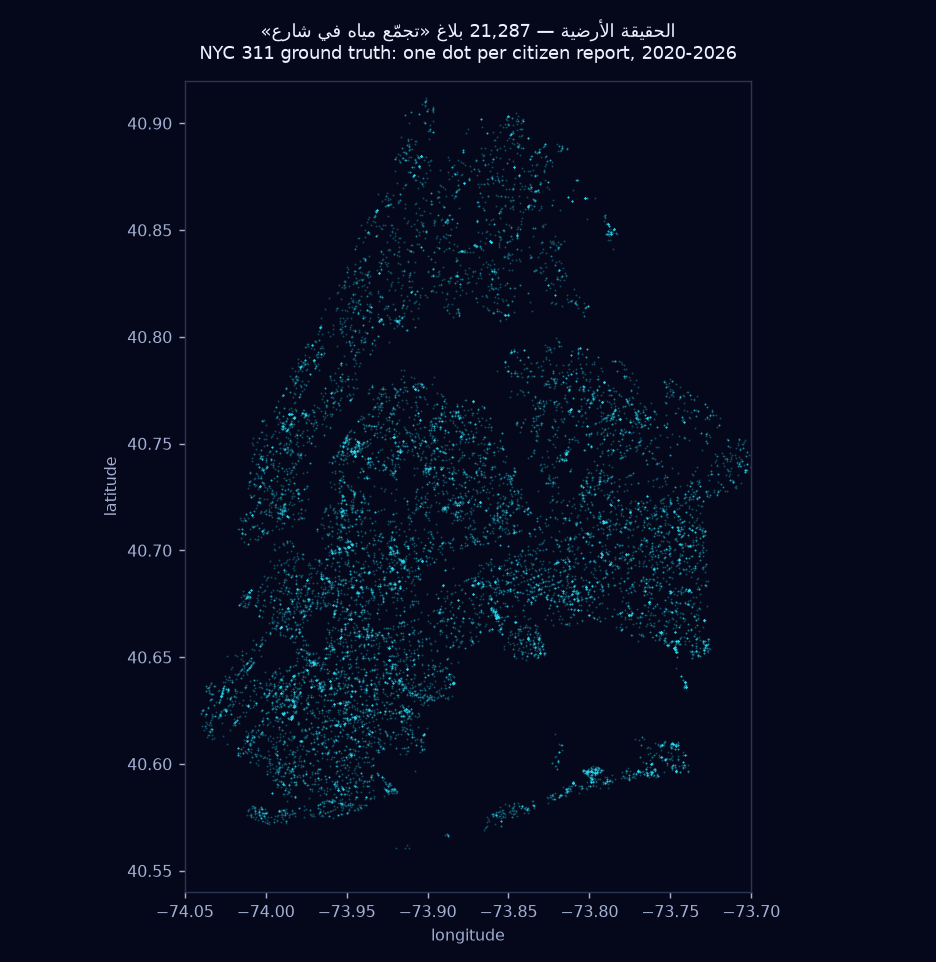
\includegraphics[width=0.7\linewidth]{figures/fig04-labels.png}
  \caption{The ground truth as it arrives. \num{21287} geolocated street-flooding
  complaints in New York City, one point per citizen report. Note the sparse centre ---
  Manhattan --- against dense Queens and Brooklyn.}
  \label{fig:labels}
\end{figure}

\subsection{Choosing the spatial unit}
Point complaints must be aggregated. \SI{200}{\metre} cells were chosen because that
approximates the length of a single street segment. Smaller cells cause a single complaint
to migrate between adjacent cells depending on geocoding precision, adding label noise;
larger cells merge streets with genuinely different behaviour into one row, diluting the
signal.

\begin{figure}[htbp]\centering
  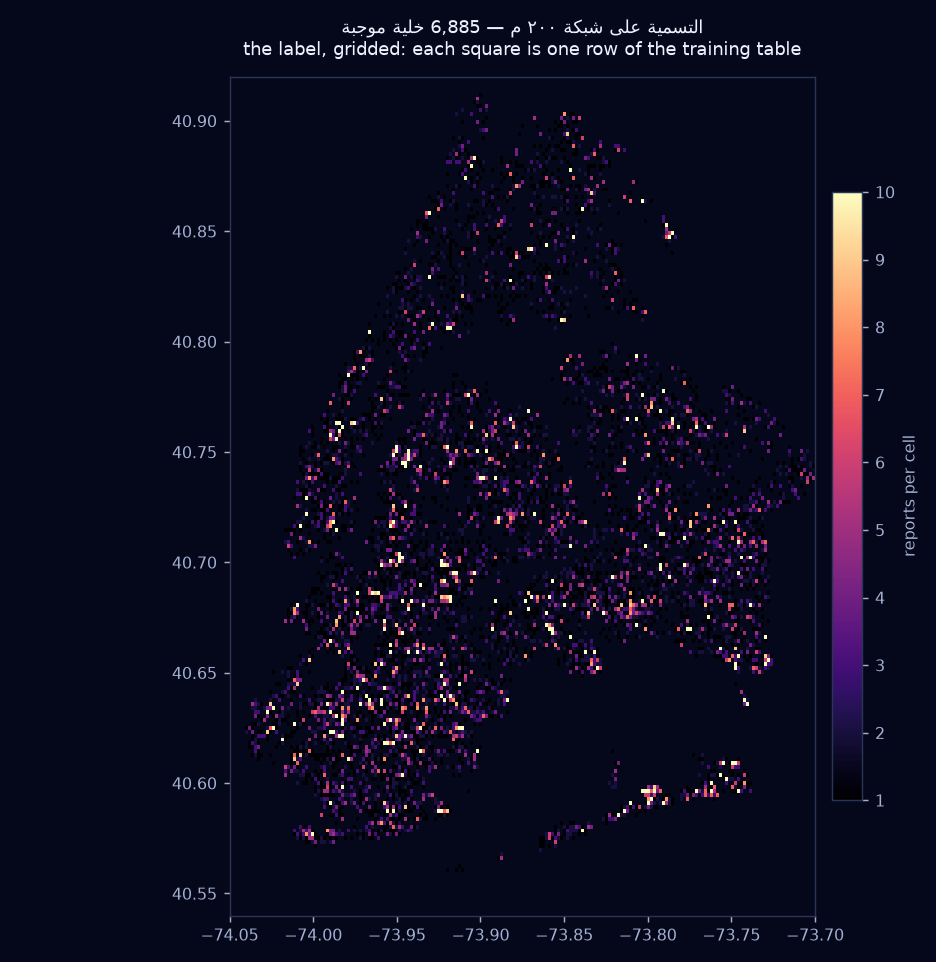
\includegraphics[width=0.7\linewidth]{figures/fig05-grid-labels.png}
  \caption{The same reports, gridded. Each \SI{200}{\metre} square becomes exactly one row
  in the training matrix, labelled 1 if any complaint fell inside it and 0 otherwise.}
  \label{fig:grid}
\end{figure}

\begin{table}[htbp]\centering\small
\caption{Final training matrix. Pooled total: \textbf{\num{62494} cells across two
cities}.}\label{tab:matrix}
\begin{tabular}{@{}lrr@{}}
\toprule
Property & New York & Chicago\\
\midrule
Analysis unit & \SI{200}{\metre} cell & \SI{200}{\metre} cell\\
Road-bearing cells & \num{25022} & \num{37472}\\
\rowcolor{rowtint}
\textbf{Prevalence} & \textbf{\SI{27.4}{\percent}} & \textbf{\SI{35.8}{\percent}}\\
Features & 9 & 9\\
Spatial CV block & $\approx\SI{5.5}{\kilo\metre}$ & $\approx\SI{5.5}{\kilo\metre}$\\
\bottomrule
\end{tabular}
\end{table}

\begin{figure}[htbp]\centering
  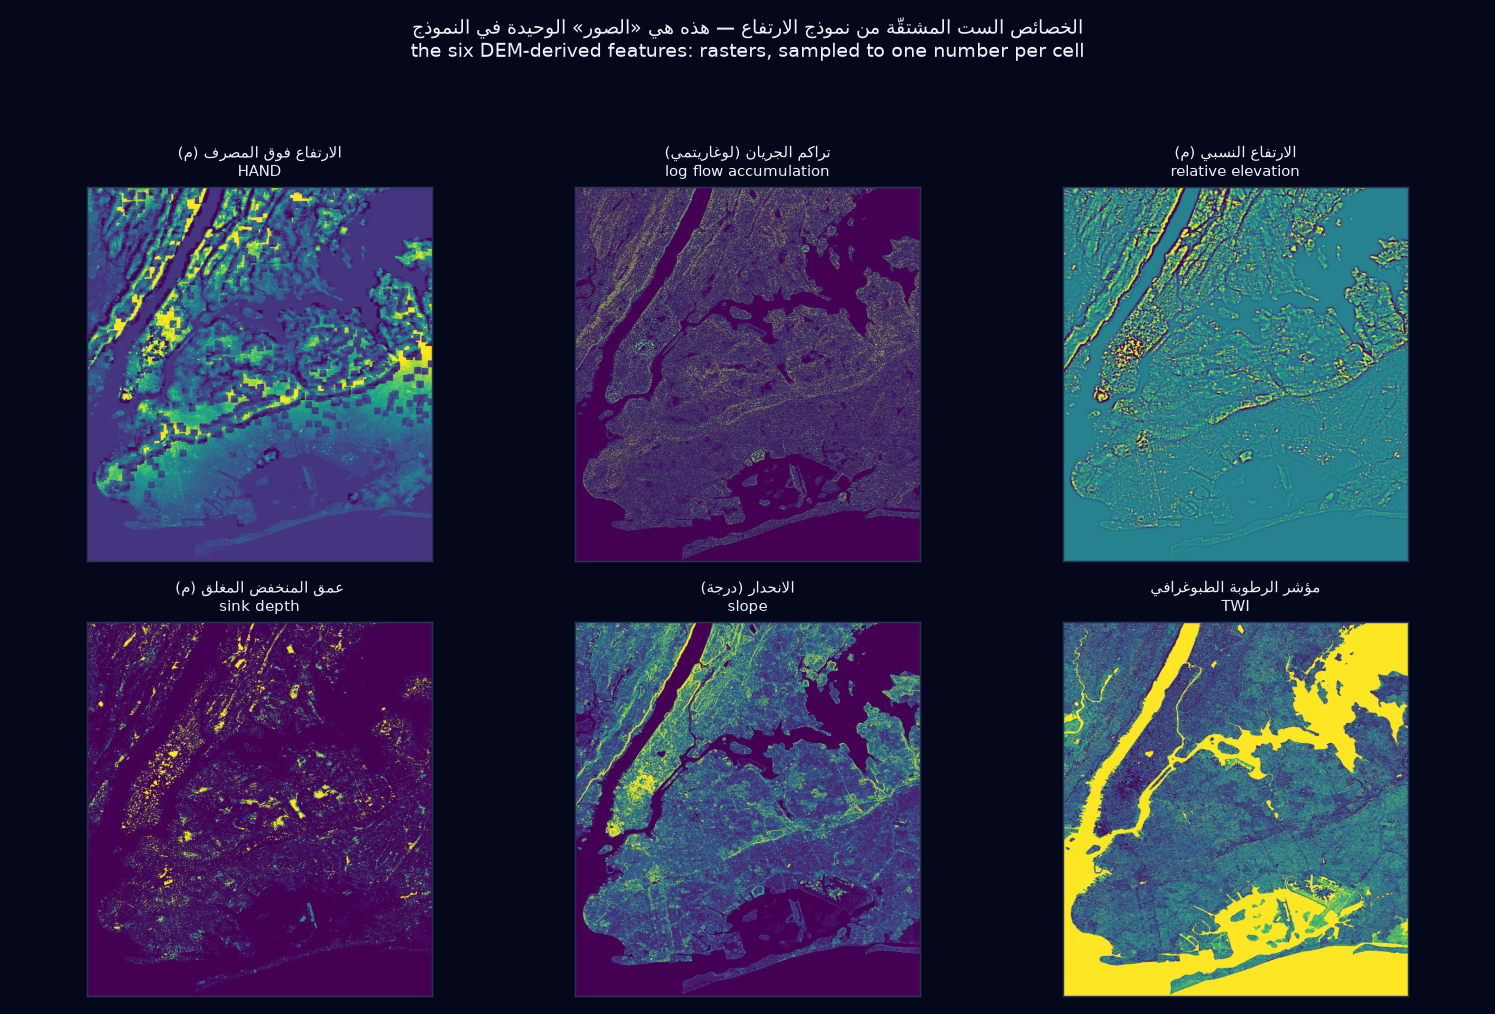
\includegraphics[width=\linewidth]{figures/fig06-feature-rasters.png}
  \caption{The six terrain features, before aggregation. Each panel is one derived
  quantity computed across the study area from the single elevation file. Every
  \SI{200}{\metre} cell reduces each surface to one number.}
  \label{fig:rasters}
\end{figure}

\subsection{The diagnostic that changed the study}
The most consequential exploratory finding was not about the features at all --- it was
about the negatives (Figure~\ref{fig:negsamp}).

\begin{figure}[htbp]\centering
  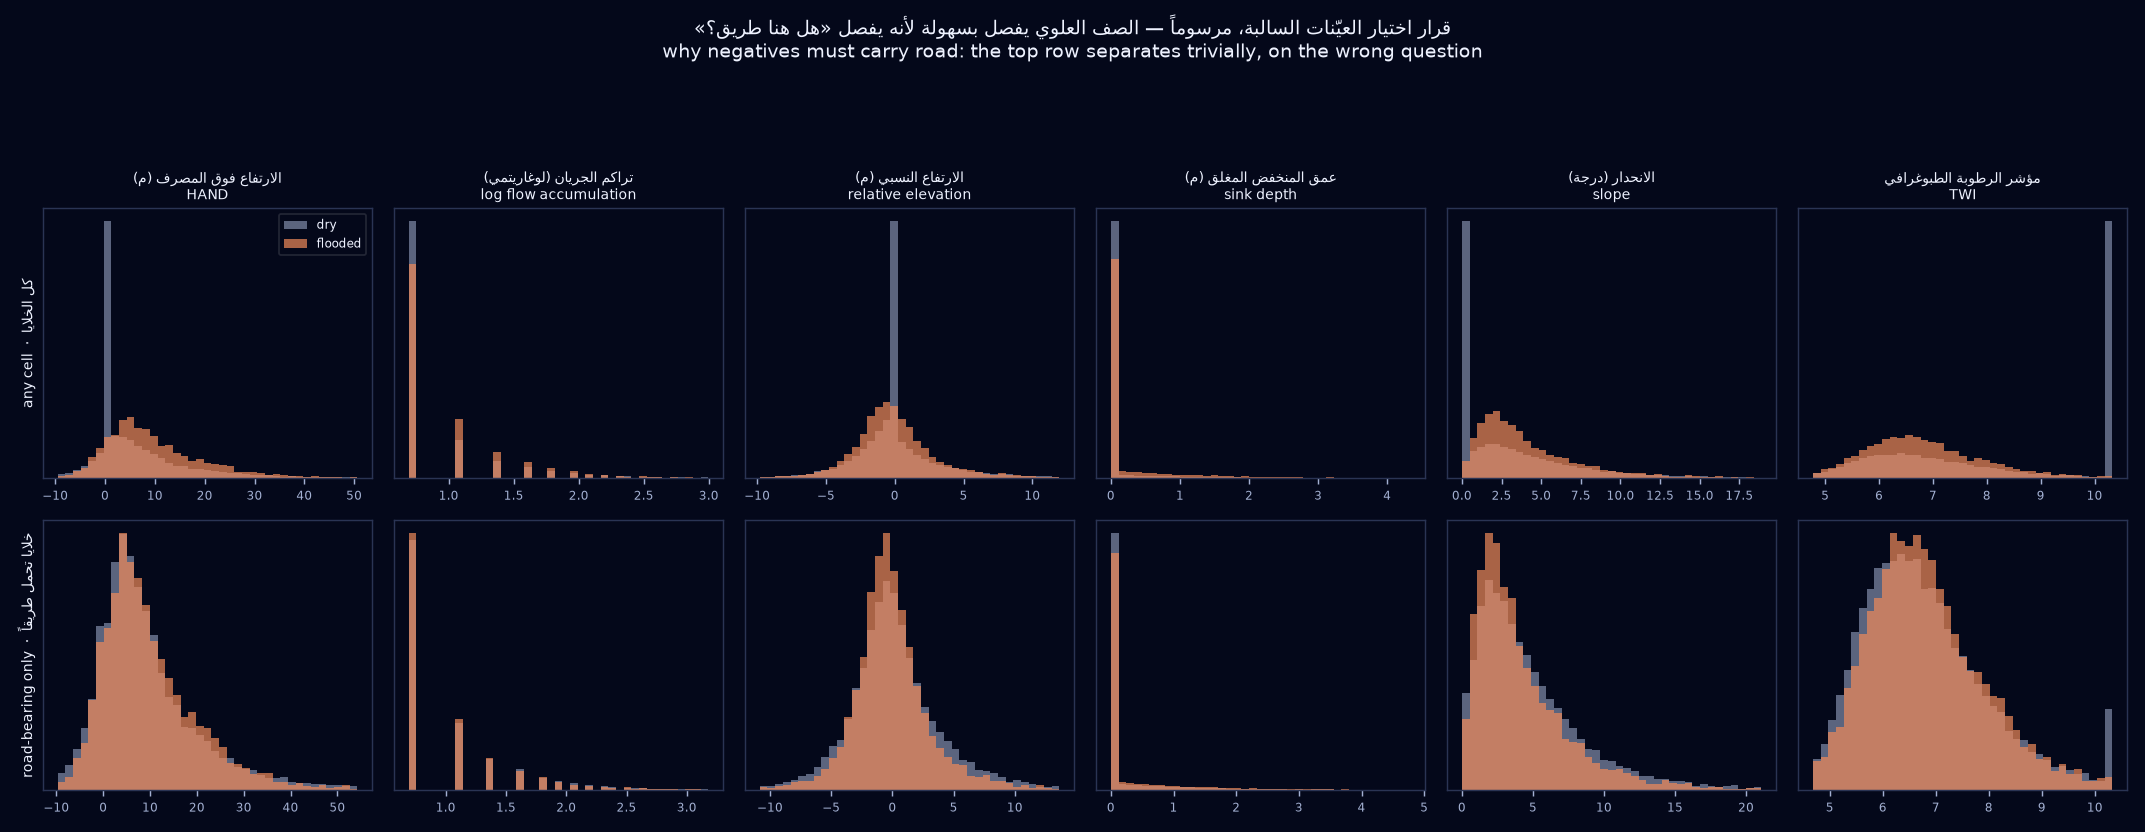
\includegraphics[width=\linewidth]{figures/fig07-negative-sampling.png}
  \caption{Why negative sampling dominated the result. \textbf{Top row:} negatives drawn
  from anywhere. The grey spikes at $\mathrm{HAND}=0$ and $\mathrm{sink}=0$ are water
  bodies, parks and vacant land, where the rasters return constant values; a model trained
  on this separates them trivially and has learned the wrong question. \textbf{Bottom row:}
  negatives drawn only from road-bearing cells (\num{34455} candidates filtered to
  \num{18162}). The spikes vanish and the distributions nearly coincide. That overlap is
  the honest reason PR-AUC is \num{0.39} rather than \num{0.9}.}
  \label{fig:negsamp}
\end{figure}

\subsection{A counter-intuitive relationship}
Binning the pooled data by road-density quintile contradicts the expectation that sparse
networks --- having less drainage --- would fare worse (Table~\ref{tab:quintiles}).

\begin{table}[htbp]\centering\small
\caption{Flooding rate by road-density quintile, pooled across both cities.}
\label{tab:quintiles}
\begin{tabular}{@{}lrrr@{}}
\toprule
Quintile & Density (km/km\textsuperscript{2}) & Flooding rate & $n$\\
\midrule
Q1 (sparsest) & 5.5 & \textbf{\SI{13.7}{\percent}} & \num{12499}\\
Q2 & 7.7 & \SI{31.4}{\percent} & \num{12499}\\
Q3 & 10.1 & \SI{35.0}{\percent} & \num{12498}\\
Q4 & 12.4 & \SI{41.8}{\percent} & \num{12499}\\
\rowcolor{rowtint}
Q5 (densest) & --- & \textbf{\SI{40.2}{\percent}} & \num{12499}\\
\bottomrule
\end{tabular}
\end{table}

The dense network floods roughly three times as often as the sparse one. The mechanism is
imperviousness: road density is a proxy for paved area, and what cannot infiltrate must
run off \citep{arnold1996}. The effect \emph{saturates} at Q5 rather than continuing to
rise, characteristic of a surface already effectively fully sealed.

%=====================================================================
\section{Feature Engineering}\label{sec:features}

\begin{figure}[htbp]\centering
  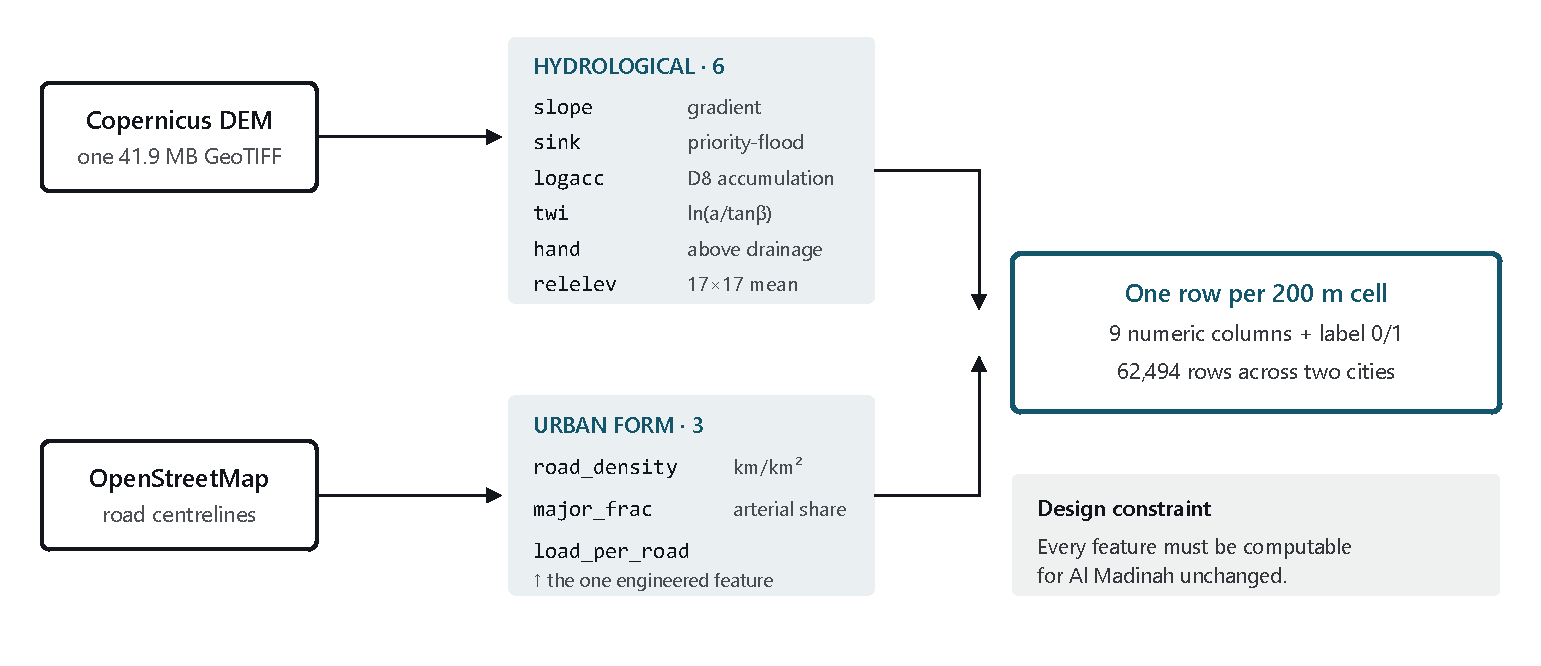
\includegraphics[width=\linewidth]{figures/fig08-feature-pipeline.pdf}
  \caption{From two open sources to one table. Six features are statistics of a single
  elevation raster; three describe road network geometry. The binding constraint on every
  one is reproducibility in the target city.}
  \label{fig:pipeline}
\end{figure}

\subsection{The hydrological six}

\paragraph{\ttt{slope} --- surface gradient (degrees).}
Steepness from the gradient of the elevation grid. Flat ground drains slowly.

\paragraph{\ttt{sink} --- closed depression depth (metres).}
The most physically direct predictor of ponding. A closed depression is a hollow with no
outlet: water that enters cannot leave except by evaporation or pumping. Depth is a
by-product of priority-flood filling \citep{barnes2014} --- the algorithm raises each pit
cell to its lowest outlet, and that rise \emph{is} the depression depth.

\begin{trapbox}[A documented bug worth recording]
The first implementation used a naive iterative fill. Across 60 sweeps it raised cells by
a maximum of \SI{6}{\centi\metre} --- meaning \ttt{sink}, the single most direct predictor
of standing water, was effectively a \textbf{dead feature}. Replacing it with a correct
priority-flood implementation produced a maximum depression depth of \SI{43.92}{\metre}.
\end{trapbox}

\paragraph{\ttt{logacc} --- flow accumulation, log-transformed.}
How many upstream cells drain through this one, by D8 routing \citep{ocallaghan1984} in
descending elevation order, then \ttt{log1p}. The transform is necessary because raw
accumulation is extremely skewed.

\paragraph{\ttt{twi} --- topographic wetness index.}
Equation~\eqref{eq:twi}, combining accumulation and slope into one number.

\paragraph{\ttt{hand} --- height above nearest drainage (metres).}
How far the point sits above the nearest channel draining it; the drainage network is
approximated as the top \SI{0.5}{\percent} of cells by flow accumulation.

\paragraph{\ttt{relelev} --- relative elevation (metres).}
$\mathrm{DEM}-(17\times17$ moving mean$)$. Purely local: is this point lower than its
immediate surroundings? It complements \ttt{sink}, which requires a fully closed
depression, by capturing shallow local lows that are not sealed.

\subsection{The urban-form three}

\paragraph{\ttt{road\_density} --- kilometres of road per km\textsuperscript{2}.}
Each centreline is densified so its length contributes to every cell it crosses. A proxy
for impervious surface, and the strongest single feature in the model.

\paragraph{\ttt{major\_frac} --- arterial share.}
Fraction of road length classified motorway, trunk, primary or secondary. Wide arterials
collect runoff from a larger area and discharge it to fewer points.

\paragraph{\ttt{load\_per\_road} --- hydraulic load per metre of road.}
\begin{equation}
\ttt{load\_per\_road} = \log\!\left(1 + \frac{\text{flow accumulation}}
{\max(\text{road length},\,25)}\right)
\end{equation}

This is the \textbf{only engineered feature}, prompted by an explicit question: does lower
road density mean more standing water? The direct answer is no
(Table~\ref{tab:quintiles}), but the question pointed at a real physical quantity ---
\textbf{load per unit of drainage capacity}. Road length is the only available proxy for
capacity, because gullies are installed along streets; flow accumulation is the load.
Their ratio has physical meaning that density alone does not express, and it ranks fifth
of nine by importance.

%=====================================================================
\section{Model Architecture}\label{sec:model}

\subsection{What gradient boosting does}
A \textbf{decision tree} splits data by threshold questions and follows branches to a
prediction; a single shallow tree is a weak model. \textbf{Boosting} builds many trees in
sequence, each fitted to the \emph{errors remaining} after all previous trees have had
their say. The final prediction sums the ensemble, and each tree contributes only a small
fraction governed by the learning rate.

\begin{figure}[htbp]\centering
  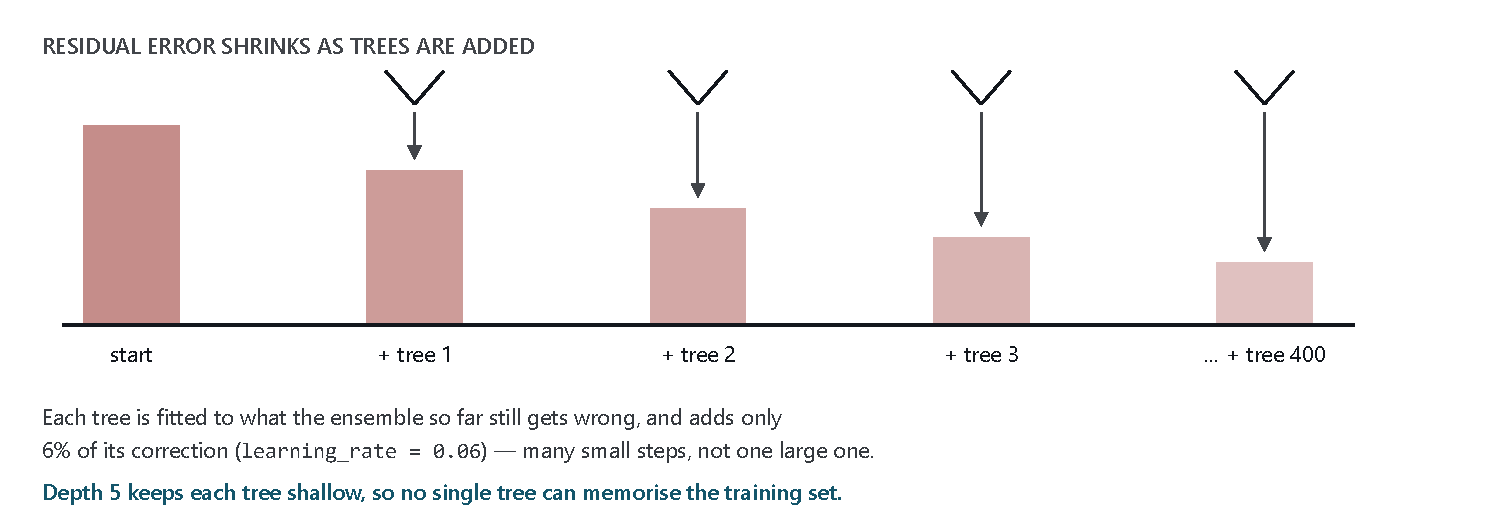
\includegraphics[width=\linewidth]{figures/fig09-boosting.pdf}
  \caption{Boosting as sequential error correction. The bars represent error remaining
  after each stage. No individual tree is accurate; the ensemble is. Shallow trees plus a
  small learning rate is the standard defence against overfitting.}
  \label{fig:boost}
\end{figure}

\subsection{Why this algorithm}
\begin{itemize}
  \item \textbf{Not logistic regression} --- relationships are non-linear. Depression depth
        matters greatly between 0 and \SI{0.5}{\metre} then saturates.
  \item \textbf{Not a neural network} --- \num{62494} rows and nine features do not justify
        one. There is no representation to learn; the features are the representation.
  \item \textbf{Gradient-boosted trees} handle non-linearity and interaction natively, need
        no feature scaling, and expose a \ttt{gain} attribution a municipal engineer can be
        shown as a reason. Auditability was a requirement, not a bonus.
\end{itemize}

\begin{table}[htbp]\centering\small
\caption{XGBoost configuration \citep{chen2016xgboost}.}\label{tab:hyper}
\begin{tabular}{@{}llp{7.0cm}@{}}
\toprule
Parameter & Value & Controls\\
\midrule
\ttt{n\_estimators} & 350 CV / 400 final & Number of trees\\
\ttt{max\_depth} & 5 & Splits root to leaf --- shallow, to limit memorisation\\
\ttt{learning\_rate} & 0.06 & Fraction of each tree's correction applied\\
\ttt{subsample} & 0.85 & Row fraction sampled per tree\\
\ttt{colsample\_bytree} & 0.85 & Feature fraction sampled per tree\\
\rowcolor{rowtint}
\ttt{scale\_pos\_weight} & $n_{\text{neg}}/n_{\text{pos}}$ & Up-weights the minority class;
  recomputed \emph{inside each fold}\\
\ttt{eval\_metric} & \ttt{aucpr} & Optimises area under the PR curve\\
\ttt{tree\_method} & \ttt{hist} & Histogram-based split finding\\
\ttt{random\_state} & 42 & Reproducibility\\
\bottomrule
\end{tabular}
\end{table}

Two choices deserve comment. \ttt{scale\_pos\_weight} is computed \emph{within each fold}
rather than once globally, because the class ratio differs between folds and a global
value would leak information across the split. And \ttt{eval\_metric} is \ttt{aucpr}
rather than the default \ttt{logloss}, so the quantity optimised during training is the
quantity reported at evaluation.

\subsection{The trained artefact}
The model ships as a single \SI{901}{\kilo\byte} file, \ttt{research/model\_pooled.joblib},
containing the classifier, the nine column names \emph{in order} (reordering them corrupts
predictions silently), the city list, \ttt{n\_train}, and \ttt{loco} --- the
leave-one-city-out transfer results.

\begin{notebox}
Storing \ttt{loco} alongside the weights is deliberate. Nobody can pick up this model and
apply it to an unseen city without simultaneously seeing what that transfer costs. The
honesty is built into the artefact rather than left to the documentation.
\end{notebox}

%=====================================================================
\section{Validation Design}\label{sec:validation}

\subsection{Choosing the negatives}\label{sec:negatives}
If negatives are drawn from anywhere on the map, they disproportionately land on parks,
water bodies, rail yards and vacant lots --- places carrying neither roads nor complaints.
Those separate trivially from flooded streets, and a model trained this way scores well
while having learned the question \emph{is there a road here?}

\begin{figure}[htbp]\centering
  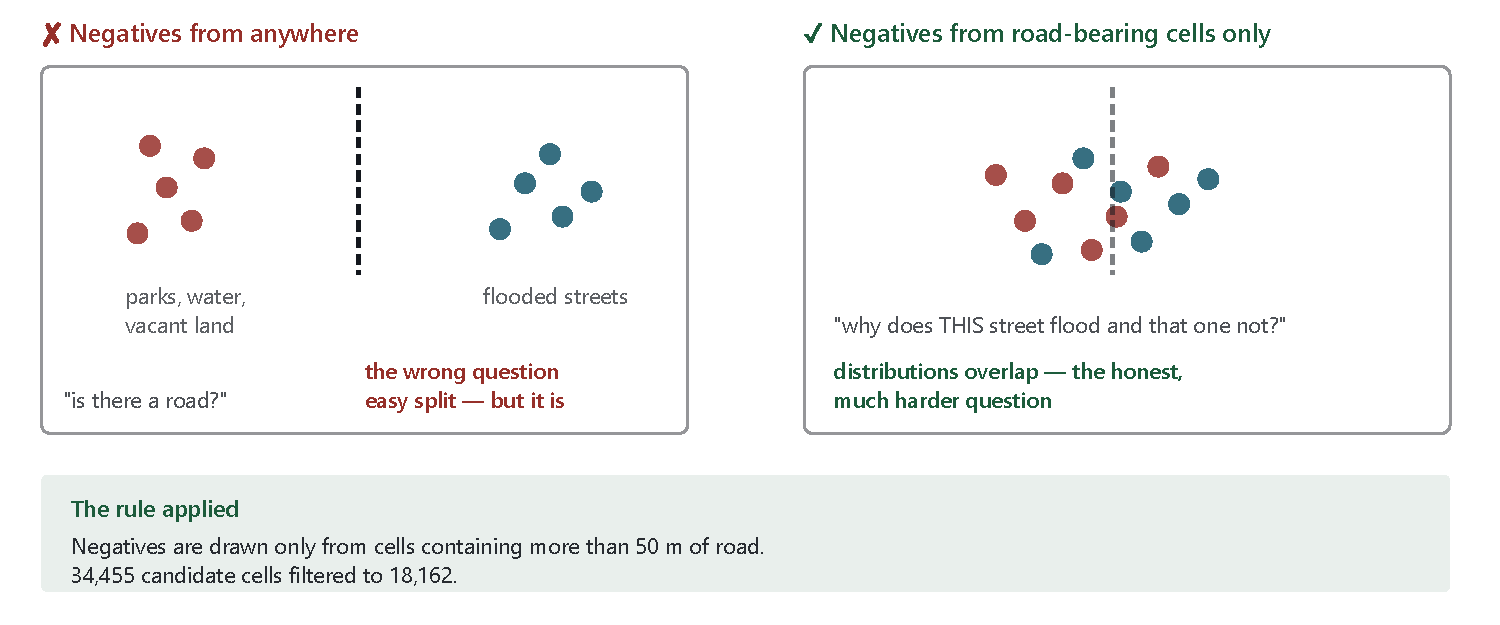
\includegraphics[width=\linewidth]{figures/fig10-negative-sampling.pdf}
  \caption{The decision that mattered more than the algorithm. Restricting negatives to
  road-bearing cells forces the classifier to explain why one \emph{street} floods and
  another does not, instead of detecting the presence of pavement. It lowers the reported
  score substantially and is the reason the score means anything.}
  \label{fig:negrule}
\end{figure}

\begin{keybox}[The rule applied]
Negatives are drawn \textbf{only} from cells containing more than \SI{50}{\metre} of road.
\num{34455} candidate cells were filtered to \num{18162}.
\end{keybox}

\subsection{Spatial blocking}
The protocol is \ttt{GroupKFold} with five folds, where the group is a contiguous spatial
block of $0.05^{\circ}\approx\SI{5.5}{\kilo\metre}$. Whole blocks are held out, so no test
cell has a training neighbour.

\begin{figure}[htbp]\centering
  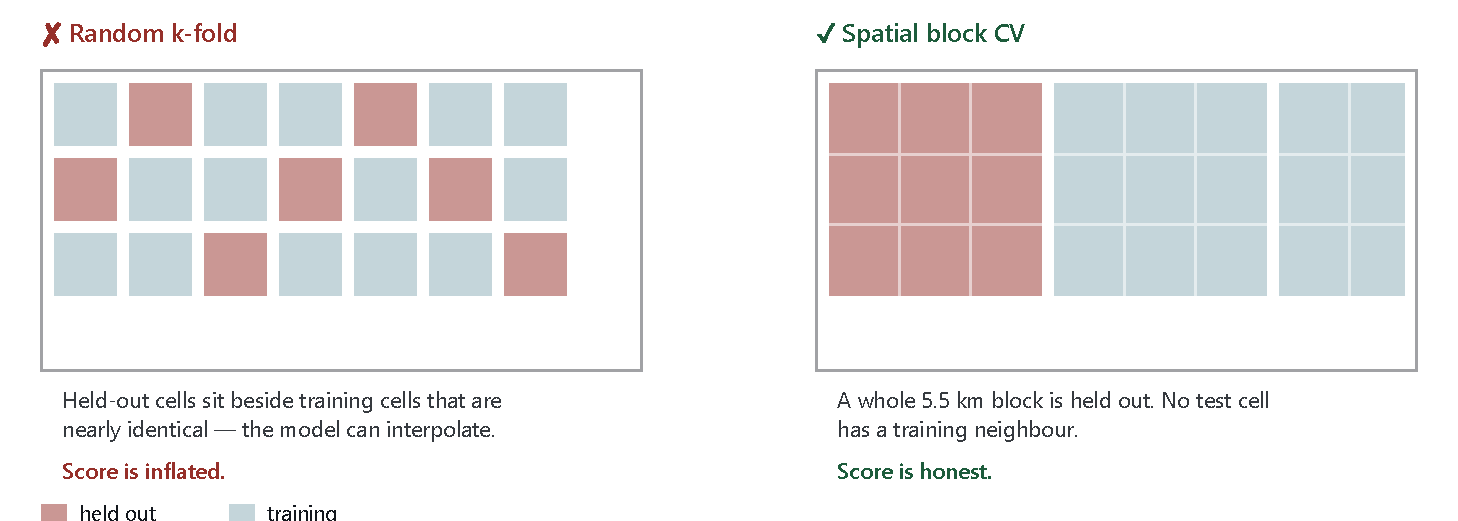
\includegraphics[width=\linewidth]{figures/fig11-spatial-cv.pdf}
  \caption{Why the split geometry changes the number. Under random $k$-fold, a held-out
  cell's neighbour --- sharing its slope, catchment and pavement --- is in the training
  set, so the model largely recognises rather than predicts. Blocking at
  \SI{5.5}{\kilo\metre} removes that shortcut.}
  \label{fig:spatialcv}
\end{figure}

\subsection{Leave-one-city-out}
Spatial blocking answers whether the model generalises across neighbourhoods; it cannot
answer whether it generalises across \emph{cities}. The decisive test is therefore
leave-one-city-out: train on Chicago, test on New York; then the reverse. Nothing about
the test city is seen during training --- not its terrain, not its labels, not its
prevalence. This is the closest available analogue to deploying on Al Madinah.

%=====================================================================
\section{Evaluation Metrics}\label{sec:metrics}

\subsection{Precision, recall, and why accuracy fails}
For a municipality, a false negative is a street that floods without being on the
inspection list; a false positive is a crew sent to a street that turns out fine. These
costs are not symmetric.

\begin{align}
\text{Precision} &= \frac{TP}{TP+FP} \\
\text{Recall} &= \frac{TP}{TP+FN}
\end{align}

Precision asks: of the streets flagged, how many really flood? Recall asks: of the streets
that flood, how many were flagged? With \SI{27.4}{\percent} of New York cells positive,
the laziest possible classifier --- one that ignores every feature and always answers
``no flood'' --- achieves $TP=0$, $FP=0$, and therefore an accuracy of
\SI{72.6}{\percent}.

\begin{trapbox}[A useless model scores \SI{72.6}{\percent}]
It finds nothing, flags nothing, and helps nobody --- and it beats many honestly
constructed models on accuracy. Any result reporting accuracy on an imbalanced problem is
reporting the class balance, not the model.
\end{trapbox}

\subsection{The precision--recall curve and the baseline}
Sweeping the decision threshold traces the precision--recall curve; the area under it,
\textbf{PR-AUC}, summarises performance across all operating points. A classifier
assigning random scores achieves, at any recall, a precision equal to the fraction of
positives. Its PR-AUC therefore equals the prevalence: \num{0.274} in New York,
\num{0.358} in Chicago.

Because the baseline differs between cities, raw PR-AUC is not comparable across them.
Dividing each by its own baseline produces a comparable quantity:

\begin{equation}
\text{lift} = \frac{\text{PR-AUC}}{\text{prevalence}}
\label{eq:lift}
\end{equation}

A lift of \num{1.0}$\times$ means no skill whatsoever.

\begin{figure}[htbp]\centering
  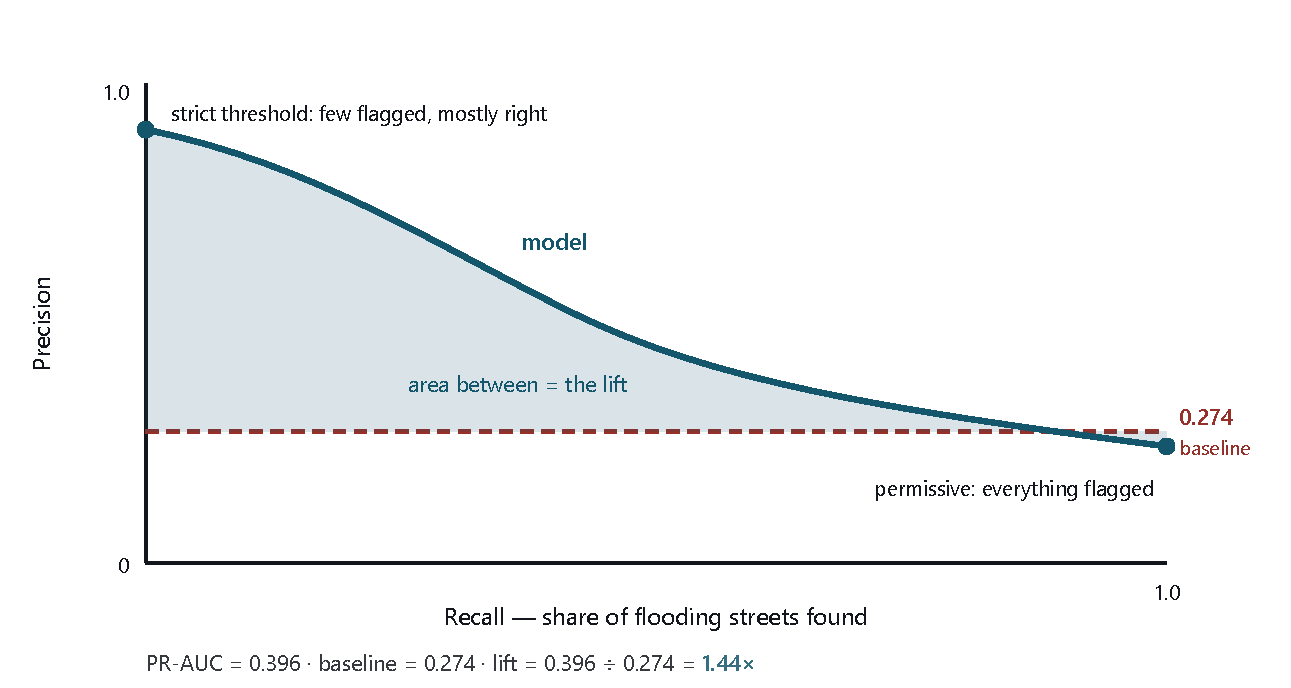
\includegraphics[width=0.84\linewidth]{figures/fig12-pr-curve.pdf}
  \caption{Reading a PR curve, and where \num{1.44}$\times$ comes from. The dashed line is
  what random guessing achieves --- a precision equal to the prevalence, \num{0.274}, at
  every recall. The area under the model's curve is \num{0.396}. The ratio is the lift.}
  \label{fig:prcurve}
\end{figure}

\subsection{ROC-AUC, and why it is secondary}
ROC-AUC plots true positive rate against false positive rate. On imbalanced data the false
positive rate has a large denominator, so substantial numbers of false alarms barely move
it \citep{davis2006,saito2015}. ROC-AUC is reported here only for comparability with a
literature that overwhelmingly uses it; no conclusion rests on it.

\begin{keybox}[Translating the metric into operations]
A lift of \num{1.24}--\num{1.30}$\times$ means inspecting the top-ranked
\SI{10}{\percent} of segments finds considerably more genuinely problematic streets than
inspecting a random \SI{10}{\percent}. \textbf{It does not mean the top \SI{10}{\percent}
are all problems.} Some flooding streets will be missed, and some highly ranked streets
will turn out fine.
\end{keybox}

%=====================================================================
\section{Results}\label{sec:results}

\begin{table}[htbp]\centering\small
\caption{Performance under 5-fold spatially blocked cross-validation.}\label{tab:within}
\begin{tabular}{@{}lrrrr@{}}
\toprule
City & PR-AUC & Baseline & Lift & Cells\\
\midrule
\rowcolor{rowtint}
New York & 0.396 & 0.274 & \textbf{1.44$\times$} & \num{25022}\\
\rowcolor{rowtint}
Chicago & 0.520 & 0.358 & \textbf{1.45$\times$} & \num{37472}\\
\bottomrule
\end{tabular}
\end{table}

The two cities agree closely despite different terrain, climate and sewer design ---
itself informative, suggesting the feature set captures something general.

\begin{table}[htbp]\centering\small
\caption{Leave-one-city-out transfer. The test city contributes nothing to training.}
\label{tab:transfer}
\begin{tabular}{@{}llrrrr@{}}
\toprule
Train & Test & PR-AUC & Baseline & Lift & ROC-AUC\\
\midrule
\rowcolor{rowtint}
Chicago & New York & 0.340 & 0.274 & \textbf{1.24$\times$} & 0.609\\
\rowcolor{rowtint}
New York & Chicago & 0.465 & 0.358 & \textbf{1.30$\times$} & 0.652\\
\bottomrule
\end{tabular}
\end{table}

Transfer costs roughly \num{0.15}--\num{0.20}$\times$ of lift relative to staying within a
city. That degradation is real and expected --- sewer design, climate and reporting
culture all change --- but performance \textbf{remains above baseline in both directions}.
A feature set that only worked one way round would suggest an artefact of one city;
working both ways is much harder to explain away.

\begin{keybox}[From claim to measurement]
Before this test, ``what transfers to Al Madinah is the shape of the model'' was an
\emph{assertion}. After it, it is a \emph{measurement} --- taken on \num{101756} field
reports across two cities, in both directions.
\end{keybox}

\begin{table}[htbp]\centering\small
\caption{Gain-based feature importance, pooled model, \num{62494} cells.}\label{tab:importance}
\begin{tabular}{@{}lrll@{}}
\toprule
Feature & Gain & Layer & Reading\\
\midrule
\rowcolor{rowtint}
\ttt{road\_density} & \SI{26.0}{\percent} & Urban & Imperviousness proxy\\
\rowcolor{rowtint}
\ttt{major\_frac} & \SI{12.9}{\percent} & Urban & Arterials concentrate runoff\\
\ttt{sink} & \SI{11.7}{\percent} & Terrain & Closed depression depth\\
\ttt{hand} & \SI{10.3}{\percent} & Terrain & Height above nearest drainage\\
\rowcolor{rowtint}
\ttt{load\_per\_road} & \SI{10.2}{\percent} & Urban & The engineered feature\\
\ttt{relelev} & \SI{9.6}{\percent} & Terrain & Local hollow\\
\ttt{logacc} & \SI{7.1}{\percent} & Terrain & Flow accumulation\\
\ttt{slope} & \SI{6.2}{\percent} & Terrain & Gradient\\
\ttt{twi} & \SI{6.0}{\percent} & Terrain & Wetness index\\
\bottomrule
\end{tabular}
\end{table}

\begin{figure}[htbp]\centering
  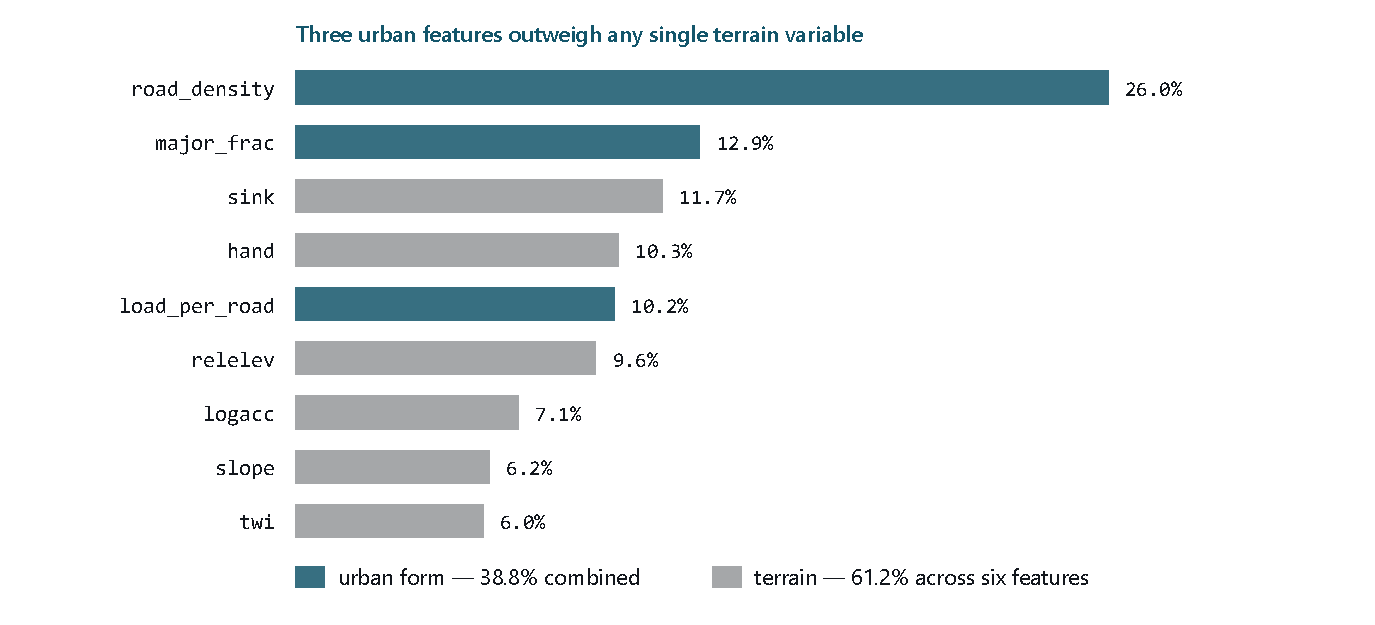
\includegraphics[width=0.88\linewidth]{figures/fig13-importance.pdf}
  \caption{The result that changed the design. Three urban-form features carry
  \SI{38.8}{\percent} of total gain --- more than any individual terrain variable --- and
  \ttt{road\_density} alone carries \SI{26.0}{\percent}.}
  \label{fig:importance}
\end{figure}

\subsection{Comparison with published work}\label{sec:compare}
\begin{limitbox}[No claim of superiority is made]
There is no agreed benchmark for this framing --- same descriptor, same cell size, same
negative-sampling rule, same validation geometry. Much of the literature reports ROC-AUC
under random splits, which is not comparable with PR-AUC under spatial blocking. A direct
numerical comparison would be misleading, so none is offered.
\end{limitbox}

The closest published work using the same New York complaints with TWI, HAND and
depression depth is \citet{kelleher2020}. The claim made here is narrow: the feature set
available for Al Madinah carries real signal under the harshest validation protocol we
know how to apply.

%=====================================================================
\section{Application to Al Madinah}\label{sec:madinah}

\begin{figure}[htbp]\centering
  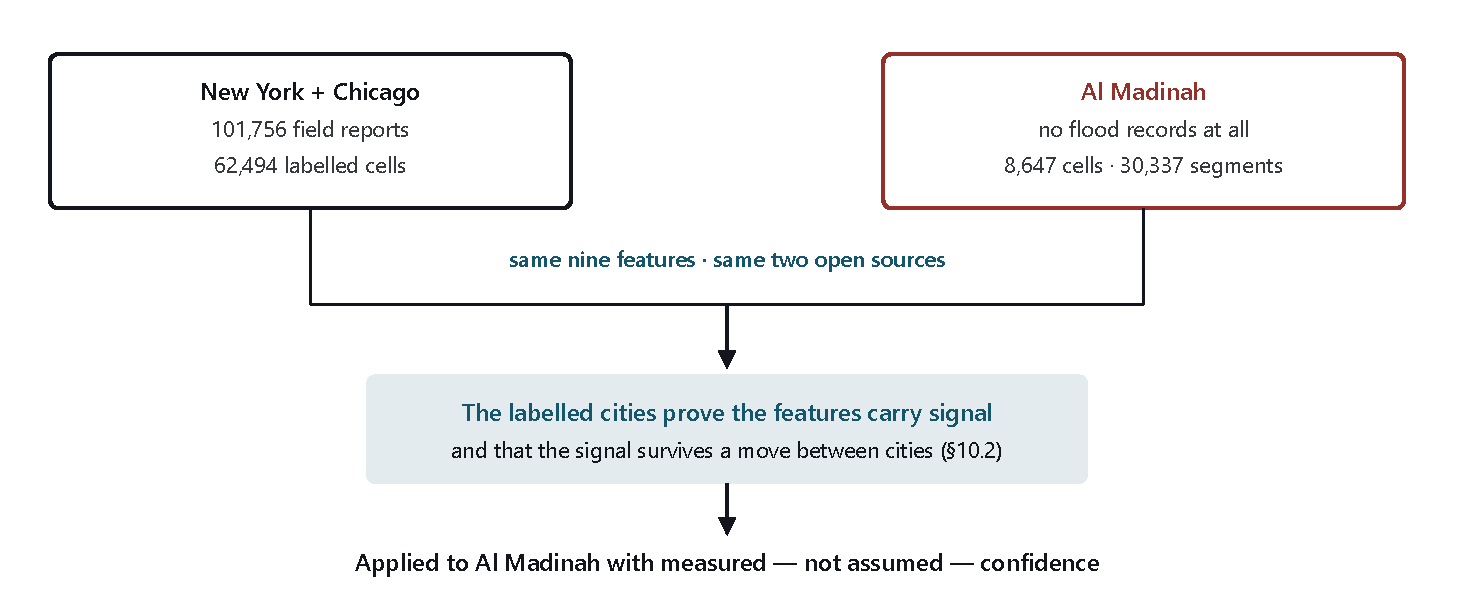
\includegraphics[width=\linewidth]{figures/fig14-transfer-logic.pdf}
  \caption{The logical order of the study. Al Madinah is never trained on and never tested
  on. It is scored by a model whose transfer cost has been measured elsewhere.}
  \label{fig:logic}
\end{figure}

\begin{notebox}
This is enforced rather than assumed: \ttt{train\_multi.py} excludes any city lacking a
\ttt{labels\_url}. Feeding \num{30000} unlabelled Al Madinah rows in as negatives would
have silently destroyed both the baseline and the transfer test at once.
\end{notebox}

\subsection{What transfers and what does not}

\begin{table}[htbp]\centering\small
\caption{The transfer boundary, stated explicitly.}\label{tab:boundary}
\begin{tabular}{@{}p{6.0cm}p{6.4cm}@{}}
\toprule
\textbf{Transfers} & \textbf{Does not transfer}\\
\midrule
The nine feature definitions & \textbf{The fitted weights}\\
The road-bearing negative rule & Decision thresholds\\
The spatial blocking protocol & Prevalence\\
Terrain relationships (physical) & Sewer design\\
 & Climate --- 30 events in 11 years\\
 & Reporting culture\\
\bottomrule
\end{tabular}
\end{table}

\subsection{Results for the city}

\begin{table}[htbp]\centering\small
\caption{Al Madinah segment classification. High + critical = \num{6068}. The top-ranked
\num{2000} span \SI{327}{\kilo\metre}, of which \SI{73}{\percent} are residential
streets.}\label{tab:bands}
\begin{tabular}{@{}lrp{7.2cm}@{}}
\toprule
Band & Segments & Recommended action\\
\midrule
\rowcolor{rowtint}
Critical & \num{1517} & Add to drainage plan; field survey before the coming season.
  Flagged \ttt{requires\_hydraulic\_engineer}\\
\rowcolor{rowtint}
High & \num{4551} & Inspect and clean surface drains before the season --- a cleaning
  truck, not a capital scheme\\
Moderate & \num{9102} & Monitor\\
Stable & \num{15167} & Explicitly excluded from the plan\\
\bottomrule
\end{tabular}
\end{table}

Within the top \num{2000} segments, 483 need only drain inspection and cleaning while
\num{1517} warrant an engineering survey. Those are enormously different budget lines, and
separating them is what turns a ranking into a plan.

\begin{trapbox}[The score is a rank, not a probability]
A score of \num{1.00} means \emph{this segment is first in the susceptibility ordering}.
It does \textbf{not} mean a \SI{100}{\percent} chance of flooding. The deployed interface
prints this on the segments page, alongside a second warning: \emph{the model does not
know where drainage networks have actually been built}. A segment ranked critical may
already have been remediated.
\end{trapbox}

%=====================================================================
\section{Limitations and Threats to Validity}\label{sec:limits}

\begin{table}[htbp]\centering\small
\caption{Known limitations.}\label{tab:limits}
\begin{tabular}{@{}p{4.2cm}p{8.4cm}@{}}
\toprule
Limitation & Consequence\\
\midrule
\rowcolor{rowtint}
\ttt{dist\_to\_drain} absent & Distance to the nearest storm drain is theoretically among
  the strongest predictors. New York publishes catch-basin locations; adding it is the
  highest-return improvement available\\
\rowcolor{rowtint}
DSM, not DTM & Buildings are in the elevation surface (\S\ref{sec:dsm}). Flow routing
  partly crosses rooftops in dense blocks --- \SI{2.44}{\metre} error at the 90th
  percentile\\
\SI{30}{\metre} resolution & New York has 1-foot LiDAR. Re-running on it would separate
  ``our features are weak'' from ``our terrain is coarse''\\
No imperviousness layer & Road density proxies for it --- a reasonable substitute, not an
  equivalent\\
No rainfall exposure term & Every cell is treated as receiving equal rain\\
\rowcolor{rowtint}
Reporting bias & Complaints come from those who complain. Part of the learned signal may
  be \emph{who reports} rather than \emph{where the problem is}\\
Elevation ends in 2015 & Construction since then is invisible, in a city that is expanding\\
\rowcolor{rowtint}
No field validation & Not one Al Madinah segment has been confirmed on the ground. This is
  the largest outstanding gap\\
\bottomrule
\end{tabular}
\end{table}

The reporting-bias limitation is recursive and deserves emphasis. The argument for this
system is that complaint-driven maintenance produces an inverted picture in which vocal
neighbourhoods appear worst. But the training labels \emph{are} complaints, so some of
that bias sits inside the model. The mitigations are partial: the road-bearing negative
rule removes the crudest confound, and the cross-city test would penalise a model that had
learned one city's reporting culture. Neither eliminates the problem; a local field
campaign is the only real remedy.

%=====================================================================
\section{Future Work}\label{sec:future}

\paragraph{Local labels --- the decisive step.}
Al Madinah weights require Al Madinah labels. Two sources are planned: (i) self-labelling
from the Sentinel-1 radar archive back to 2014, where every historical rain event can in
principle yield a flooded/not-flooded label per segment with no fieldwork; and (ii) a field
verification campaign with the municipality on a sample of top-ranked segments after a rain
event. With either, the model can be retrained locally and Al Madinah becomes a
contributor rather than a consumer.

\paragraph{Model improvements, in order of expected return.}
Add \ttt{dist\_to\_drain}, validated first on New York where catch-basin locations are
published; re-run on FABDEM or LiDAR to quantify how much residual error is terrain
coarseness rather than feature weakness; add an imperviousness layer to separate the
paved-surface effect from the road-geometry effect currently conflated in
\ttt{road\_density}.

\paragraph{Independent impact measurement.}
Over eight million linear metres of drainage have been laid nationally with no independent
instrument measuring whether individual schemes worked. Because the satellite archive is
retrospective, a before/after comparison is possible for projects already commissioned ---
a capability requiring no new data collection.

%=====================================================================
\section{Conclusion}\label{sec:conclusion}

Al Madinah has no record of where its streets flood. That absence is normally treated as a
reason not to attempt prediction, or as something to work around quietly while reporting a
confident accuracy figure. This work took the constraint as the research question instead.

The signal is real and it does transfer, at a measured cost. Nine features derived from one
free elevation file and one open street map achieve \num{1.44}$\times$ and
\num{1.45}$\times$ over baseline within cities under spatially blocked validation, and
\num{1.24}$\times$ and \num{1.30}$\times$ when moved to a city never seen in training.
Along the way the data contradicted two expectations: urban form outweighed terrain, and
dense street networks flooded three times as often as sparse ones.

What this produces for a municipality is not certainty. It is a ranked list of \num{30337}
street segments, each with a written reason and a suggested action, covering streets nobody
has ever complained about --- available before the season rather than after the storm. For
an authority responsible for \SI{5280}{\kilo\metre} of network with finite crews, replacing
complaint-driven triage with a ranking of measured lift is a real gain.

The honest summary is the one the interface itself prints: the number is a rank, not a
probability; the model does not know where drainage has already been built; and no segment
in Al Madinah has yet been confirmed on the ground. Those three sentences are part of the
claim, not caveats appended to it.

%=====================================================================
\section*{Data and Code Availability}
\addcontentsline{toc}{section}{Data and Code Availability}
All input data is open: Copernicus DEM GLO-30 from a public AWS bucket, OpenStreetMap via
Overpass, and the New York and Chicago 311 archives via Socrata. The full experiment
rebuilds from raw sources with a single containerised command invoking
\ttt{build\_city.py} for each city followed by \ttt{train\_multi.py}; feature computation
for Al Madinah uses \ttt{madinah\_features.py} and scoring uses \ttt{score\_madinah.py}.

%=====================================================================
\bibliographystyle{plainnat}
\bibliography{refs}

\end{document}
